\documentclass[nojss]{jss}
\usepackage[sc]{mathpazo}
\usepackage{geometry}
\geometry{verbose,tmargin=2.5cm,bmargin=2.5cm,lmargin=2.5cm,rmargin=2.5cm}
\setcounter{secnumdepth}{2}
\setcounter{tocdepth}{2}
\usepackage{breakurl}
\usepackage{hyperref}
\usepackage[ruled, vlined]{algorithm2e}
\usepackage{mathtools}

\usepackage{float}
\usepackage{placeins}
\usepackage{mathrsfs}
\usepackage[toc,page]{appendix}
\usepackage{multirow}
\usepackage{amsmath}
\usepackage{breqn}
\usepackage[demo]{graphicx}% "demo" to make example compilable without .png-file
\usepackage{pdflscape}
\usepackage{lipsum}

\usepackage{booktabs}
\newcommand{\head}[1]{\textnormal{\textbf{#1}}}
%% \usepackage{mathbbm}
\DeclareMathOperator{\sgn}{sgn}
\DeclareMathOperator*{\argmax}{\arg\!\max}

\title{\bf faoswsFisheryStandardization: Methodological proposal and workflow}

\author{Francesca Rosa\\ Food and Agriculture
    Organization \\ of the United Nations\\}

\Plainauthor{Francesca Rosa}

\Plaintitle{faoswsFisheryStandardization: Methodological proposal and workflow}

\Shorttitle{Fisheries SUA/FBS}

\Abstract{

  This document provides an overall description of the methodology developed to compile FBS in the Fishery domain. It is the result of a continuous interaction between FIAS and SWS teams. It covers almost all the steps to compile FBS starting from unbalanced SUA equations.
  This document also contains explicit references to the \pkg{faoswsFisheryStandardization} repository and to the SWS objects (dataset, datatables) involved in the process. \\

}

\Keywords{Food Balance Sheets, Supply Utilization Account Equations}
\Plainkeywords{Capture, Aquaculture, Commodity Tree, Standardization}


\usepackage{Sweave}
\begin{document}
\Sconcordance{concordance:faoswsFisheryStandardization.tex:faoswsFisheryStandardization.Rnw:%
1 50 1 1 0 262 1 1 37 9 0 1 2 250 1}

\SwaveParseOpstions


\section {Introduction}
FIAS SWS domain hosts several datasets. Fishery data has been split in different datasets in order to reproduce the data structure already in place in the current FIAS dissemination system (FishStatJ).

The following list contains the list of all the SWS datasets stored in the Fisheries SWS data domain\footnote{At the time this documentation has been written, not all the datasets included in this list have been created and properly populated in the SWS. In addition, the mesioned datasets are all related to the FIAS FBS. Both \textit{Vessel} and \textit{Dispositions} dataset are included in the Fisheries domain, but are not included in the FBS workflow.}: 

\begin{itemize}
\item{Global Production, given by the aggregation on two components:}
  \begin{itemize}
    \item {Capture}
    \item {Aquaculture}
  \end{itemize}
\item{Global Production (Frozen), a perfect clone of the just introduced \textit{Globla Production} dataset that is used as input to compile FBS.}  
\item{Commodity DB, containing trade data and the production associated to processed and preserved items.}
\item{SUA (Supply and Utilization Account) tables, both unbalanced and balanced};
\item{FBS (Food Balance Sheets) tables,  containing SUA \textit{standardized}, in other words SUAs equations whose components have been aggregated and expressed in their primary equivalent.}
\end{itemize}

The following flow charts contain an high level descrption of the workflow to compile FIAS FBS. It is mainly focused on the SWS datasets and their interactions\footnote{Appendix 1, contains a legenda to properly interpret the flow-chart shapes.}.

In the following sections will be presented a broader discussion about the key steps  to compile balanced SUA equations and subsequently FBS.

\begin{figure}
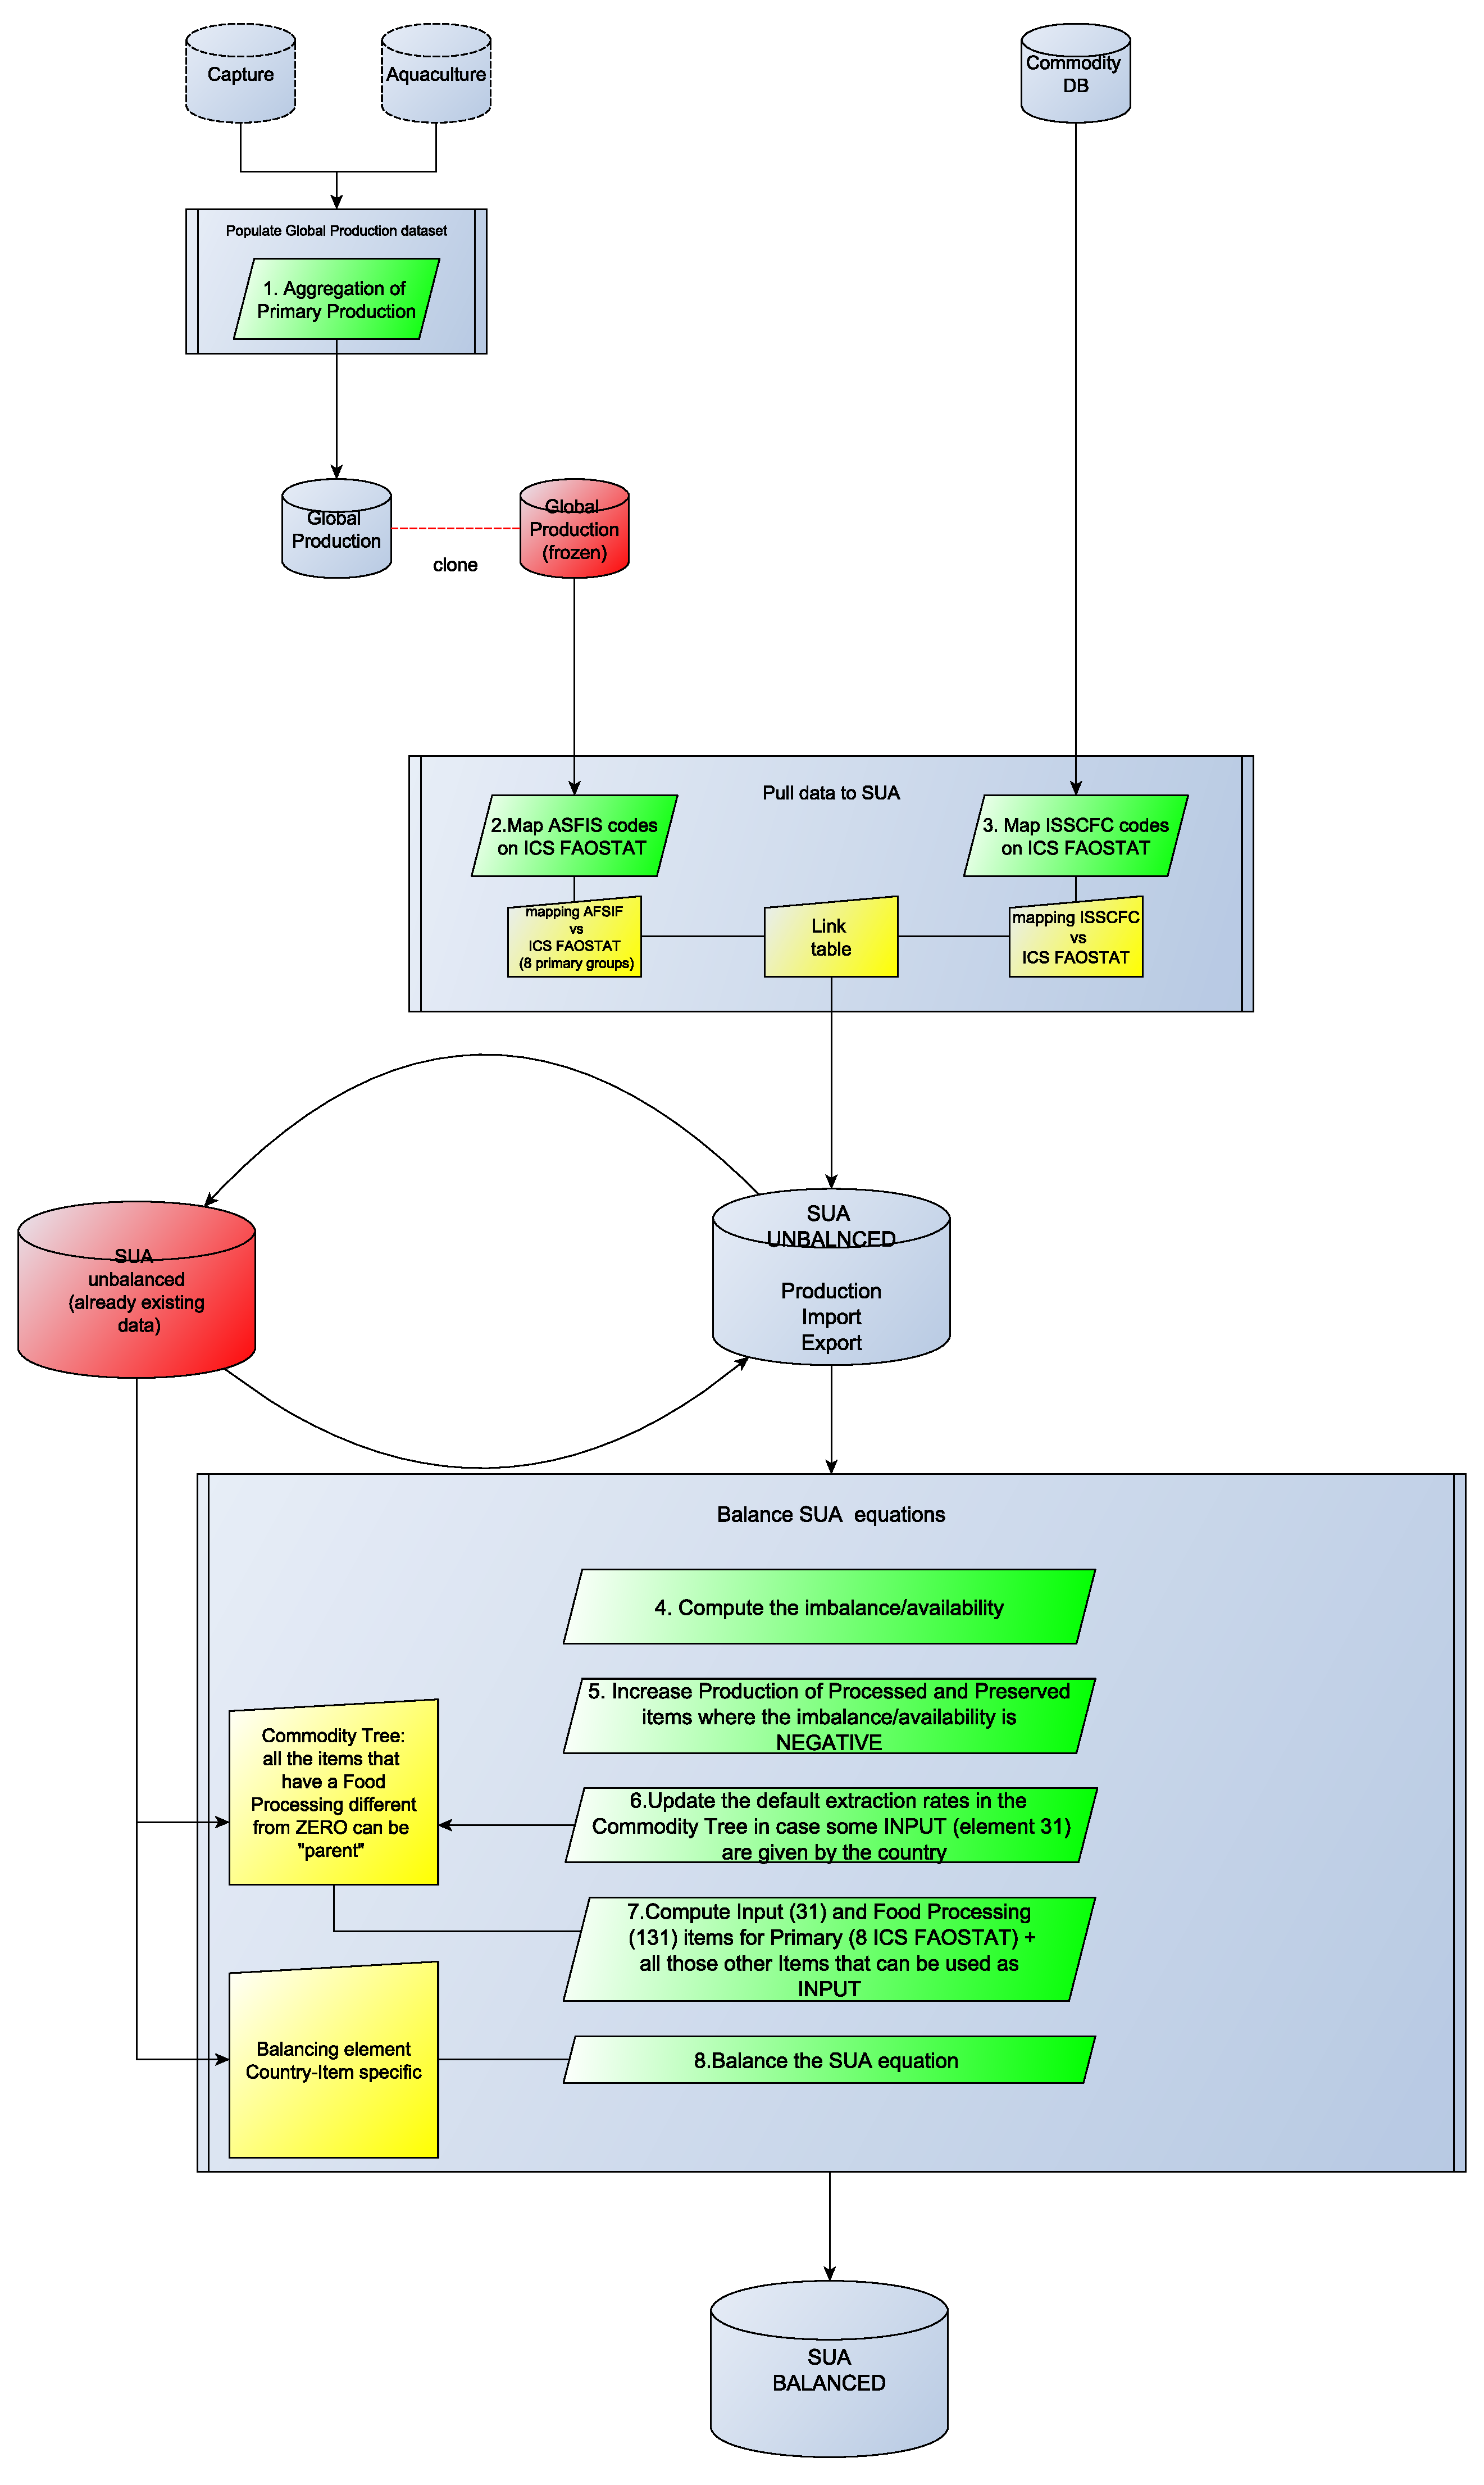
\includegraphics{flow-charts/pullDataToSUA/pullDataToSUA_globalProdFROZEN.pdf}
\caption{Overall workflow}
\end{figure}




\section {FIAS datasets - migration to the SWS}

\subsection{Global Production}
Primary Production data for Fishery products may come from both Capture and Aquaculture. Capture and Aquaculture data are collected and stored in two different SWS datasets. Data is collected via FIAS questionnaire and it is consolidated and fully validated thanks an intense activity of research on the web and on official publications.

The Global Production data set is considered reliable enough to be autonomously disseminated. It basically represents the starting point to compute FBS and, together with the Commodity DB (see Section 2.2.) it is used to compile the primary availability, which is the amount of primary product allocated as input for any productive processes which lead to the production of processed and preserved items.

Both capture and aquaculture data are collected according to the ASFIS list of Species for Fishery Statistics Purposes. 

\paragraph{Primary production - ASFIS classification}

For each species, the following descriptors are provided: 

\begin{itemize}
\item \textbf{3-alpha code}: classification issues only for species of commercial significance. Its codes have a predefined structure: three alphabetic characters that represent a very short abreviation of the name of the species\footnotes{ It is used in tables, questionnaires and publications in which the lack of space may impede the use of adequate descriptors in all the languages}. FAO is the depository agency for the 3-alpha codes: all requests for information and for the allocation of a 3-alpha code to new species should be addressed to FAO. 


\item \textbf{Taxonomic code}: hierachical classification consisting of five levels of aggregation (Main groupings, Orders, Families, Genera and Species). It contains also several attributes for each code: scientific name, author(s), family \dots
\end{itemize}

All species in the ASFIS list are classified by \textbf{ISSCAAP group}, with the exception of marine birds and snakes. The International Standard Statistical Classification for Aquatic Animals and Plants (ISSCAAP) classifies aquatic commercial species into 50 groups and nine divisions on the basis of their taxonomic, ecological and economic characteristics. The ISSCAAP groups are used to aggregate ASFIS items into macro-categories and to finally map ASFIS codes onto ICS FAOSTAT groups.


\paragraph{Aggregation of Capture and Aquaculture into the Global Production dataset - }
Capture and Aquaculture datasets are consistent in terms of classifications, but are not completely consistent in terms of dataset dimensions. Aquaculture has one more data dimension: Production Source (brackishwater, freshwater, marine)\footnote{Note that the term dimension is used the identify the dataset columns whose combintion univocally identifies a data-point.}.
Once both Capture and Aquaculture data have been validated, the two datasets are aggregated to populate the Global Production SWS dataset. 
This procedure includes the following steps:
\begin{itemize}
\item Aggregate the Aquaculture data by ''Production source'' in order to remove the dimension ''Production Source'' and make the both Aquaculture and Capture dataset compliant in terms of dataset-dimentions.
\item Furtherly aggregate by species the amount of production  coming from Capture with the amount coming from Aquaculture in order to have, at country level, one unique figure referring to the primary production for each species by fishing Area, on a yearly basis.

\end{itemize}
The routine to properly aggregate Capture and Aquaculture dataset has been already uploaded in the SWS (as a R plugin). It has been developed by FIAS teams\footnote{Thomas Berger is the focal point - plugin in Prod env: \textit{Global Production}.}.

As shown in the \textit{Overall workflow} flowchart, \textit{Global Production} dataset (obtained as result of the this aggregation) is frozen and cloned. The cloned \textit{Global Production} dataset is a separate envirnoment and it is a perfect copy of the \textit{Global Production} dataset currently released. This step ensures to FIAS team to keep working on the Global Production dataset without interfeering with the activities related to the FBS compilation. This latter version of the \textit{Glabal Production} dataset which is fully validated, released and frozen, is used as input to produce the FBS. This dataset has the structure reported in Table 1.

\subsection {The Commodities DB}
The socalled  Commodities database contains mainly trade data, anyway it also contains production of processed and preserved commodities \footnote{For a comprehensive discussion about the Commodity DB and its production component, make reference to the document \textit{Production of processed and preserved items in the Commodity DB}}.

Items are classified according to the International Standard Statistical Classification of Fisheries Commodities (ISSCFC). It covers products derived from fish, crustaceans, molluscs and other aquatic animals, plants and residues. This classification is based on the structure of the United Nations Standard International Trade Classification (SITC), with additional codes to include links to ISSCAAP and breakdown by additional species and product forms. It includes links to the Harmonized System classification (HS) and to the Central Product Classification (CPC). In the ISSCFC, fisheries and aquaculture commodities are classified according to the species and to the degree of processing undergone.

As aready mentioned, this dataset (together with the Primary Production) is used as input to the FBS compilation. While the trade components (Import and Export) are cosidered relieable enough and cannot be modified by the Standardization procedure\footnote{Procedure to convert all the processed }, the Production component of the Commodity Database can be readjusted.

\begin{landscape}
\begin{table}[t]
\caption{Global Production - dataset structure}
\centering
\begin{tabular}{c|c|c|c|c|c|c|c}
\toprule
geographicAreaM49 & fisheriesAsfis & fisheriesCatchArea & measuredElement & timePointYears & Value & flagObservationStatus & flagMethod\\
\midrule

itme1 & 36.101954 & 45 & 0.825500 & 0.220198 & 0.293448 & x & y \\
item2 & 51.828572 & 45 & 0.224900 & 0.499718 & 0.690064& x & y \\

\bottomrule
\end{tabular}
\label{tab:xxx}
\end{table}


\end{landscape}



\subsection{SUA unbalanced}
Once \textit{Global production} and \textit{Commodity DB} data has been reconciled, production and trade flows, properly associated to \textit{ICS FAOSTAT} groups, populate the \textit{SUA unbalanced} table.

The R routine to update the already existing SUA tables is generally referred as the \textit{Pull data to SUA}\footnote{Please note that the \textit{Pull Data to SUA} operation is currently the first part of the routine developed to compile FBS}.

Given that the SUA had been already compiled in the past, the socalled SUA unbalanced table, actually contain the SUA equations that had been already balanced at least up to the last release of the FBS. In other words, the first time the SUA unbalanced table is popultaed, existing SUA tables (already balanced) should be included in the SWS dataset. 

Each time the \textit{Pull data to SUA} routine is run, the updated figures are highlighted (red triangle in the corner of the cell) and the user can easily visualize which figures had changed.


The migration of current SUAs tables into the SWS request the mapping of the current element codes onto the SWS element list. Table 2. contains the first draft proposal to convert current FIAS SUAs into the SWS SUA unbalanced table.


\begin{table}[t]
\caption{Proposal: mapping of the current FIAS element codes onto the SWS element codes.}
\centering
\begin{tabular}{c|c|c|c}
\toprule
FIAS code  & label & proposed code & proposed label                    \\
\midrule

51   &	Production     & 5510 & Production                             \\
61   &	Imports - Qty  & 5610 & Import Quantity [t]                    \\
62   &	Imports - Val  &   &
91   &	Exports - Qty  & 5910 & Export Quantity [t]                    \\
92   &	Exports - Val  &      &                                        \\
                  
101   &	Feed           & 5520 & Feed [t]                               \\
111   &	Breed/Bait     &      &                                        \\
                  
121   &	Waste          &    5016 & Waste [t]                           \\
131   &	Processing     &    5023 & Processed [t]                       \\
141   &	Food           &    5141 & Food [t]                            \\
151   &	Other Util     &    5166 & Residual other uses [t]             \\
                  
31   &	Input          &                     &                         \\
41   &	Extr Rate      &                     &                         \\ 

71   &	Stock Variation   &   5071 & Stock Variation [t]               \\
77   &	Cumulative Stocks &        &                                   \\

261   &	Food: Total Calories Eqv  &     &                  \\ 
264   &	Calories/Caput/Day        & 664 & Food supply (/capita/day)[kcal] \\             
271   &	Food: Total Proteins Eqv  &     &                  \\    
274   &	Proteins/Caput/Day        &     &                  \\      
281   &	Food: Total Fats Eqv      &     &                  \\    
284   &	Fats/Caput/Day            &     &                  \\    

\bottomrule
\end{tabular}
\label{tab:xxx}
\end{table} 





\section {The methodology}


The overall workflow to compile Food Balance Sheets fosees several R plugins that populate different SWS datasets or a single plugin that dave in different datasets intermediate output (\textit{sua unbalanced}, \textit{sua balanced}, \textit{fbs standardized} and any other intermediate output that might be useful for validation purposes). This choice should facilitate the data-validation procedure. The FBS officer can check the output of each sub-module and eventually manually interveene if ad hoc adjustements are required. 


The following sessions are addressed to provide details about the R modules under develpment to trasform the input data (\textit{Primary Production} dataset and the \textit{Commodity DB} into the \textit{Fishery Food Balance Sheets}).



\subsection{Populate the SUA unbalanced table: the ICS FAOSTAT classification}
To build the Supply-Utilization Account dataset, it is necessary to reconcile the information coming from the Primary Production and from the Commodity Database. Items, in these two datasets, are classified according to different classifications, ASFIS and ISSCFC respectively. This means that \textit{primary production}  and \textit{trade} data are characterized by a different level of detail in terms of species classification.

On the other hand, SUA equations are associated to ICS FAOSTAT groups. This means that fish and fish products contained in each ICS item do not represent individual species or commodities, but the aggregation of different species and products. About 2 000 species produced and 1 000 items traded are conveyed into 8 main groups of similar biological characteristic \footnote{Currently the SUAs/FBS for aquatic plants are not calculated (with the exception of three countries in FAOSTAT) due to the lack of separate data for edible/non-edible trade until recently. Due to the improvement of the HS classification and the introduction of specific codes distinguishing edible from non-edible aquatic plants/seaweed, this could change in the near future.}, reflecting the ISSCAAP classification,  with further breakdowns associated to processed and preserved commodities.

The main eight groups of species forming SUAs and FBS for fish and fishery products are: 
\begin{itemize}
\item Freshwater and Diadromous fish;
\item Demersal fish;
\item Pelagic fish;
\item Marine fish other; 
\item Crustaceans; 
\item Molluscs, excluding cephalopods; 
\item Cephalopods; 
\item Other aquatic animals.
\end{itemize}

These eight ICS groups are looked as primary items: there is a one to one relationship between between the primary ICS groups and the final  FBS groups. Table 3. shows this one to one correspondence.

\begin{table}[t]
\caption{ICS - FBS mapping}
\centering
\begin{tabular}{c|c|c}
\toprule
geographicAreaM49 & fisheriesAsfis & fisheriesCatchArea \\
\midrule

       010 &  1501    & Freshwater and Diadromous fish; \\
       020 &  1514    & Demersal fish;                  \\ 
       030 &  1527    & Pelagic fish;                   \\
       040 &  1540    & Marine fish other;              \\
       050 &  1553    & Crustaceans;                    \\
       060 &  1562    & Molluscs, excluding cephalopods \\  
       070 &  1570    & Cephalopods;                    \\
       090 &  1594    & Other aquatic animals.          \\

\bottomrule
\end{tabular}
\label{tab:xxx}
\end{table}


\begin{figure}
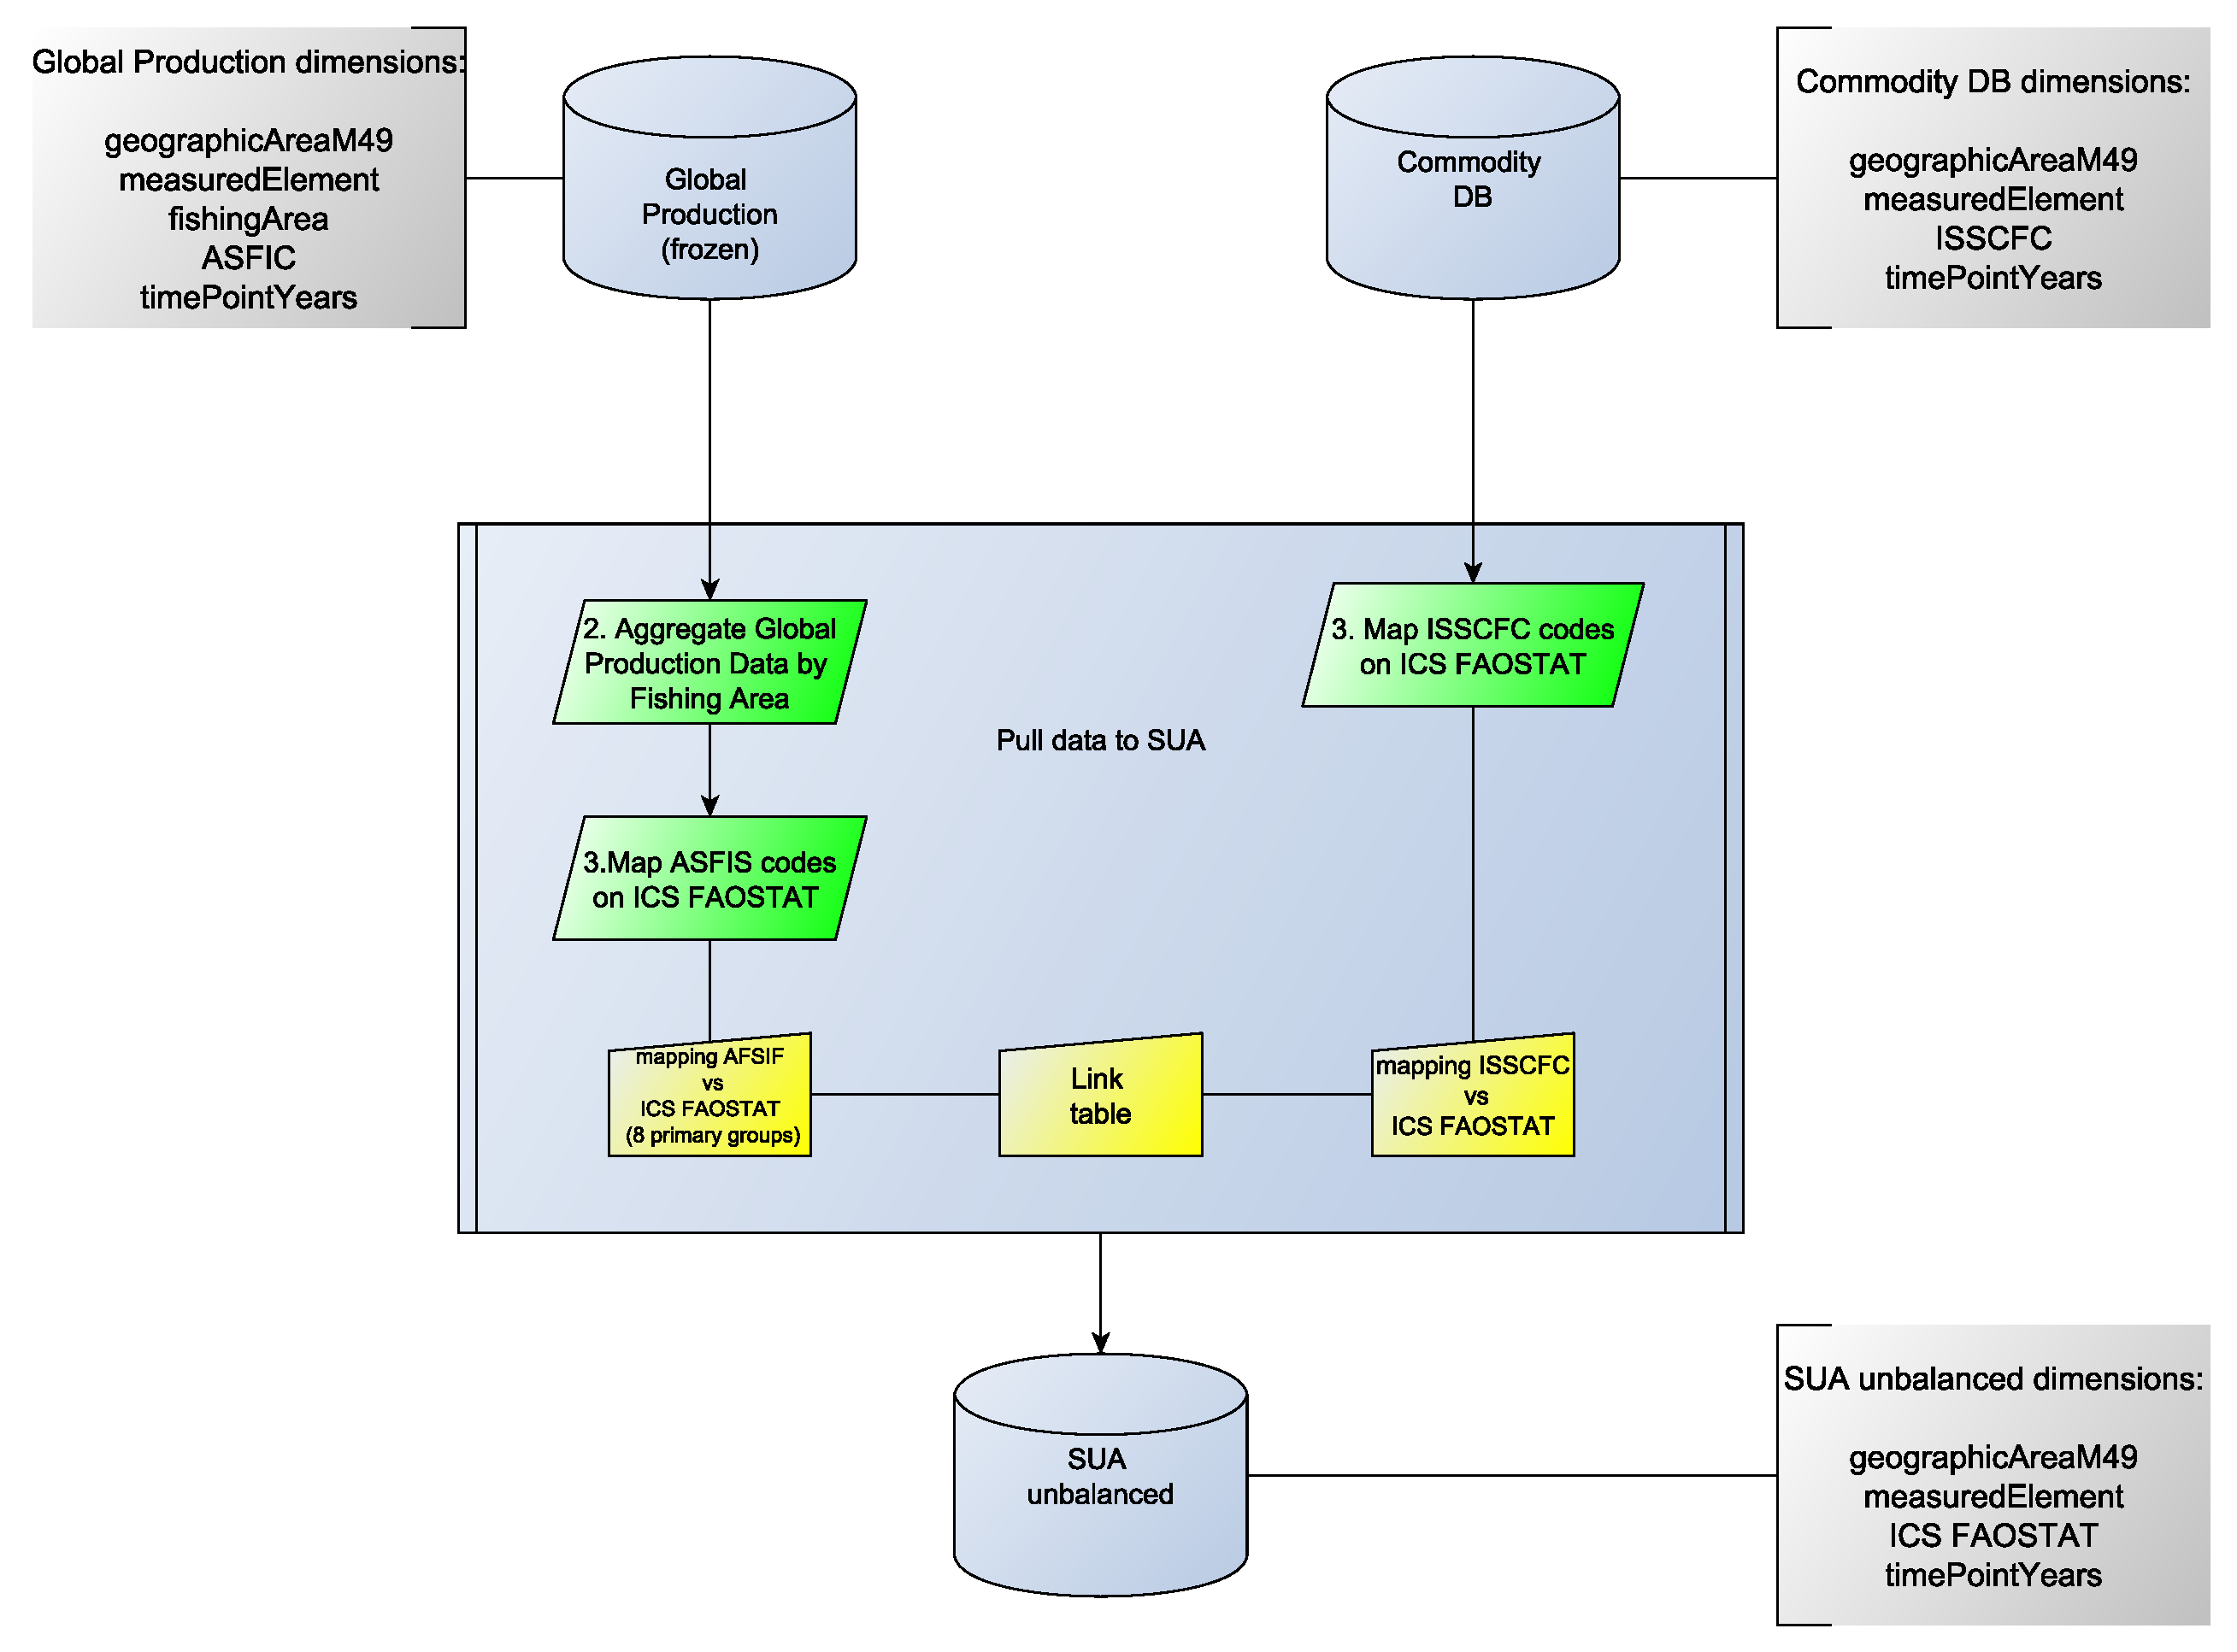
\includegraphics{flow-charts/pullDataToSUA/focusOnCompileSUA_Unbalanced.pdf}
\caption{Pull data to SUA: reconcile Global Production Data with the Commodity DB.}
\end{figure}


Figure 2. summarizes the overall workflow and reports the auxiliary-files (generally stored as data-tables in the SWS) to perform the mapping. The proper mapping tables, had been built to aggregate Primary Items (ASFIS) into the 8 primary ICS groups and the \textit{Commodity DB} items (ISSCFC) into the proper ICS group.

\paragraph{Example: ASFIS - ICS mapping}

Table 4. contains an example refferring to the composition in terms of ASFIS codes of the ISSCAAP group \textit{Carps, barbels and other cyprinids (11)} for Russia - 2014. The table also shows how all the ASFIS items associated to the eleventh ISSCAAP group are aggregated into the ICS group \textit{Freshwater & diadromous fish, fresh}(1501):

\begin{landscape}
\begin{table}[t]
\caption{ICS - FBS mapping}
\centering
\begin{tabular}{c|c|c|c|c|c|c}
\toprule
geographicAreaM49 & fisheriesAsfis & measuredElement & timePointYears & Value & isscaap & ics \\
\midrule
643   &  ABK    & 5510 & 2014 &   7193   & 11 &  1501 \\
643   &  ASU    & 5510 & 2014 &   424    & 11 &  1501 \\ 
643   &  BKC    & 5510 & 2014 &   0      & 11 &  1501 \\
643   &  CGO    & 5510 & 2014 &   0      & 11 &  1501 \\
643   &  FBM    & 5510 & 2014 &   20673  & 11 &  1501 \\
643   &  FBR    & 5510 & 2014 &   3908   & 11 &  1501 \\  
643   &  FCC    & 5510 & 2014 &   0      & 11 &  1501 \\
643   &  FCG    & 5510 & 2014 &   19468  & 11 &  1501 \\
643   &  FCP    & 5510 & 2014 &   63249  & 11 &  1501 \\
643   &  FCY    & 5510 & 2014 &   30498  & 11 &  1501 \\ 
643   &  FID    & 5510 & 2014 &   5930   & 11 &  1501 \\
643   &  FRO    & 5510 & 2014 &   758    & 11 &  1501 \\
643   &  FRX    & 5510 & 2014 &   17603  & 11 &  1501 \\
643   &  FSC    & 5510 & 2014 &   2751   & 11 &  1501 \\  
643   &  FTE    & 5510 & 2014 &   1134   & 11 &  1501 \\
643   &  SRE    & 5510 & 2014 &   8872   & 11 &  1501 \\
643   &  SVC    & 5510 & 2014 &   23315  & 11 &  1501 \\

\bottomrule
\end{tabular}
\label{tab:xxx}
\end{table}
\end{landscape} 



\subsubsection{The Link table}

Sometimes the default mapping tables do not provide the proper aggregations of ASFIS or ISSCFC codes into ICS groups. This means that some already agreggated flows have to be migrated from the default ICS group to an ad hoc one. These exceptions are counry- year specific and a data-table \footnote{domain: fisheries, datatable: \textit{link_mapping}} has been created to host this information in a such a way as to be easily digest by the R script on one hand, and easily read and updated by any FIAS user on the other.


The \textit{deviation} of any ICS aggregated flow to another, is typically based on a one to one relationship. Anyway, sometimes it is necessary to split the aggregated ICS flow into two or more alternative ICS groups. One to many relationships need an additonal information: the percentage to split one ICS flow into many\footnote{Embedded in the R routine there are also several checks to ensure that the sum of these percentage by \textit{from_code} always sum to one. }.  This additional information is contained in the \textbf{Link table} whose extraction of few lines is here reported:


